\section{CONTROL DIFFERENTIAL DRIVE MOBILE ROBOT}
\hspace{1.27cm}
There are multiple ways to control the mobile robot, namely, reference position control and reference trajectory control —etc. In this project, the robot movement is control by the trajectory tracking control based on the back-stepping technique.\par
\subsection{Kinematic Control Model}

\hspace{1.27cm}
% Figure Image =============================================================================
\begin{figure}[ht]
	\centering
	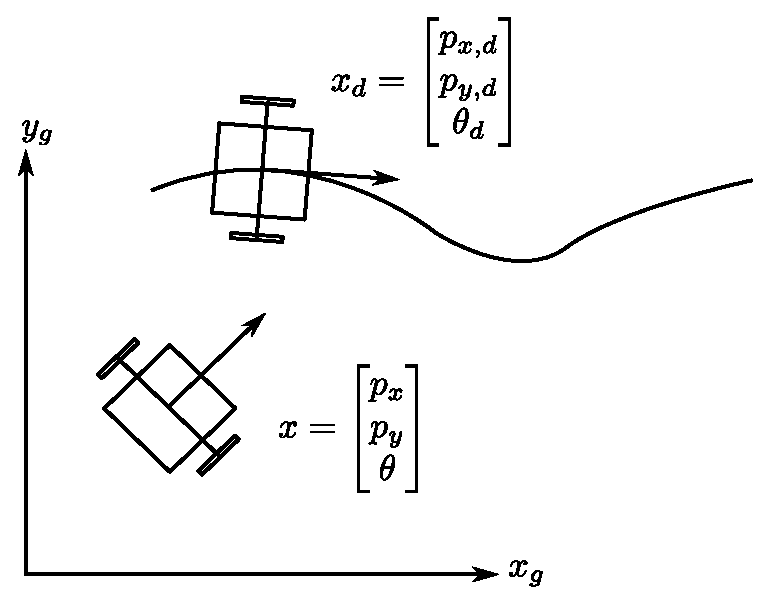
\includegraphics[scale=1]{images/imagess/5cont-kinematic.eps} 
	\caption{Differential Drive Kinematic control}
	\label{fig:Differential Drive Kinematic control}
\end{figure}
% Figure Image =============================================================================

\textbf{\figureautorefname{ \ref{fig:Differential Drive Kinematic control}}} shows the robot pose inside the environment. Let :
\begin{itemize}
	\item {\makebox[1cm]{\(x\)\hfill} represents the current pose of the robot in a time step}
	\item {\makebox[1cm]{\(x_d\)\hfill} represents the desired trajectory of the robot}
	
%    \item \(x\) represents the current pose of the robot in a time step
%    \item \(x_d\) represents the desired trajectory of the robot to move on
\end{itemize}
The purpose of the back-stepping trajectory tracking control controller is to nullify the error between the \(x\) and \(x_d\). The error between the current pose and the desired trajectory pose is defined as:

\begin{equation} \label{eq:control_error}
x_e = T \Tilde{x}
\end{equation}

Where:
\begin{equation}
x_e =
\begin{bmatrix}
e_1\\
e_2\\
e_3
\end{bmatrix}
\end{equation}

\begin{equation}
T = \begin{bmatrix}
cos\theta && sin\theta && 0\\
-sin\theta && cos\theta && 0\\
0 && 0 && 1
\end{bmatrix}
\end{equation}

\begin{equation}
\Tilde{x} = \begin{bmatrix}
p_{x,d} - p_x\\
p_{y,d} - p_y\\
\theta_d - \theta
\end{bmatrix}
\end{equation}

Taking the derivative of \ref{eq:control_error}, we obtain:
\begin{equation}
\Dot{x}_e=
\begin{bmatrix}
\Dot{e}_1\\
\Dot{e}_2\\
\Dot{e}_3
\end{bmatrix}=
\begin{bmatrix}
-1\\
0\\
0
\end{bmatrix}V+
\begin{bmatrix}
e_2\\
-e_1\\
-1
\end{bmatrix}\omega+
\begin{bmatrix}
V_{ref} cos e_3\\
V_{ref} sin e_3\\
\omega_{ref}
\end{bmatrix}
\end{equation}

Proving by the Lyapunov stability (\cite{zidani2015backstepping}), the controllers produce the control input for the robot are:
\begin{equation}
\begin{bmatrix}
V_c\\
\omega_c
\end{bmatrix} = 
\begin{bmatrix}
V_{ref} cos e_3 + k_1e_1\\
\omega_{ref} + k_2 V_{ref} e_2 + k_2 sin e_3
\end{bmatrix}
\end{equation}

Where:
\begin{itemize}
	\item {\makebox[2cm]{\(k_1,k_2,k_3\)\hfill} are the positive constants for tuning}
	\item {\makebox[2cm]{\(V_c\)\hfill} is a linear velocity control}
	\item {\makebox[2cm]{\(\omega_c\)\hfill} is an angular velocity control}
	
%	\item \(k_1,k_2,k_3\) are the positive constants for tuning
%	\item \(V_c\) is a linear velocity control 
%	\item \(\omega_c\) is an angular velocity control
\end{itemize}






\subsection{Dynamics Control Model}
\hspace{1.27cm}
Using the dynamics model of the robot, reformulate in terms of tracking control. By using coordinate transformation. Let:
\begin{equation}
\begin{split}
x_1 &= V\\
x_2 &= \omega\\
u_V &= \tau_1 + \tau_2\\
u_\omega &= \tau_1 - \tau_2
\end{split}
\end{equation}

Where:
\begin{itemize}
	\item {\makebox[2cm]{\((x_1,x_2)^T\)\hfill} is the state vector}
	\item {\makebox[2cm]{\((u_V,u_\omega)^T\)\hfill} is the control vector}
	
%    \item \((x_1,x_2)^T\) is the state vector
%    \item \((u_V,u_\omega)^T\) is the control vector
\end{itemize}

We get:
\begin{equation}
\Dot{x_1} = \frac{1}{mr}u_V
\end{equation}
\begin{equation}
\Dot{x_2} = \frac{L}{2rI}u_\omega
\end{equation}
There are two steps in this approach:\\
$\bullet$ \textbf{Step 1}:\par
Let \(x_{1ref}\) be the linear velocity of the reference trajectory. The linear velocity tracking error is defined as:
\begin{equation}
z_1 = x_{1ref} - x_1
\end{equation}
Taking the derivative of \(z_1\), we get: 
\begin{equation}
\Dot{z}_1 = \Dot{x}_{1ref}-\Dot{x}_1 = \Dot{x}_{1ref} - \frac{1}{mr} u_V
\end{equation}
From the Lyapunov function stability, we get:
\begin{equation} \label{eq:control_uV}
u_V = mr[\Dot{x}_{1ref} + k_az_1]
\end{equation}

\break
$\bullet$ \textbf{Step 2}:\par
Let \(x_{2ref}\) be the angular velocity of the reference trajectory. The angular velocity tracking error is defined as:
\begin{equation}
z_2 = x_{2ref} - x_2
\end{equation}
Taking the derivative of \(z_2\), we get:
\begin{equation}
\Dot{z}_2 = \Dot{x}_{2ref}-\Dot{x}_2 = \Dot{x}_{2ref} - \frac{L}{2rI} u_\omega
\end{equation}
From the Lyapunov function stability, we get:
\begin{equation} \label{eq:control_uomega}
u_\omega = \frac{2rI}{L}[\Dot{x}_{2ref} + k_bz_2]
\end{equation}

We have:
\begin{equation} \label{eq:control tau 1c}
\tau_{1c} = \frac{1}{2}[u_V+u_\omega]
\end{equation}
\begin{equation} \label{eq:control tau 2c}
\tau_{2c} = \frac{1}{2}[u_V-u_\omega]
\end{equation}

Substitute \ref{eq:control_uV} and \ref{eq:control_uomega} into \ref{eq:control tau 1c} and \ref{eq:control tau 2c}, we get:
\begin{equation}
\tau_{1c} = \frac{1}{2}[mr[\Dot{x}_{1ref} + k_az_1]]+\frac{2rI}{L}[\Dot{x}_{2ref} + k_bz_2]]\\
\end{equation}
\begin{equation}
\tau_{2c} = \frac{1}{2}[mr[\Dot{x}_{1ref} + k_az_1]]-\frac{2rI}{L}[\Dot{x}_{2ref} + k_bz_2]]
\end{equation}

Where:
\begin{itemize}
	\item {\makebox[1cm]{\(\tau_{1c}\)\hfill} is the control torque for the left wheel}
	\item {\makebox[1cm]{\(\tau_{2c}\)\hfill} is the control torque for the right wheel}
	\item {\makebox[1cm]{\(k_a\)\hfill} is a positive constant}
	\item {\makebox[1cm]{\(k_b\)\hfill} is a positive constant}
	
%	\item \(\tau_{1c}\) is the control torque for the left wheel
%	\item \(\tau_{2c}\) is the control torque for the right wheel
%	\item \(k_a\) is a positive constant
%	\item \(k_b\) is a positive constant
\end{itemize}






\break
\subsection{Sensor Fusion}
\hspace{1.27cm}
Sensor fusion is the method of combining the data from the sensor to determine the state of the system. One of the sensor fusion algorithms is Kalman Filter. It is an algorithm that estimates of the unknown or uncertain variable given the observation. The state of the system (in this case, the robot pose) is represented as vector with some mixed in noise (considered as ground truth). In every discrete time step, the new state is determined in the function of previous state and inputs using an operator. Then, another operator determines the measurable output (observation) from the true system. This algorithm can only apply to the linear system. Since the mobile robot is a nonlinear system, another variance of Kalman Filter is used called Extended Kalman Filter. (\cite{al2015multiple}) (\cite{moore2016generalized}). The state transition model and the measurement model in EKF are defined as :\par
\begin{equation}
    x_k = f(x_{k-1},u_{k-1}) + w_{k-1}
\end{equation}
\begin{equation}
    y_k = h(x_k) + v_k
\end{equation}

EKF is divided into two steps: the \textbf{Prediction step} and the \textbf{Correction step}.
% Table ====================================================================================
\begin{table}[h]
    \begin{center}
		\caption{Extended Kalman Filter Algorithm (\cite{kim2018introduction})}
		\label{Table: Extended Kalman Filter Algorithm}
		\begin{tabular}{lll}
		\hline
		Prediction                  && \\
		\hline
		Predicted State estimate    && \(\hat{x}^-_k = f(\hat{x}^-_{k-1},u_{k-1})\) \\
		Predicted error co-variance && \(P^-_k = JF_{k-1}P^+_{k-1}JF^T_{k-1} + Q\)\\
		\hline
        Correction                  && \\
        \hline
        Measurement predict         && \(\hat{y}_k = h(\hat{x}^-_k)\)\\
        Measurement residual        && \(\Tilde{y}_k = y_k - \hat{y}_k\)\\
        Kalman Gain                 && \(K_k = P^-_kJH^T_k(R+JH_kP^-_kJH^T_k)^{-1}\)\\
        Updated state estimate      && \(\hat{x}^+_k = \hat{x}^-_k + K_k\Tilde{y}\)\\
        Updated error co-variance   && \(P^+_k = (I-K_kJH_k)P^-_k\)\\
		%\hline
		\ChangeRT{1.5pt} 
       \end{tabular}
  \end{center}
\end{table}
% Table ====================================================================================

The superscript - and + represents the variable prior and posterior to the estimate state in the time update and the measurement update, respectively.

From \textbf{\tableautorefname{ \ref{Table: Extended Kalman Filter Algorithm}}},
\begin{itemize}
	\item {\makebox[1cm]{\(x\)\hfill} is the state vector}
	\item {\makebox[1cm]{\(P\)\hfill} is the error co-variance}
	\item {\makebox[1cm]{\(y\)\hfill} is the measurement vector}
	\item {\makebox[1cm]{\(k\)\hfill} is the time step}
	\item {\makebox[1cm]{\(u\)\hfill} is the control input vector}
	\item {\makebox[1cm]{\(w\)\hfill} is the guassian white noise}
	\item {\makebox[1cm]{\(v\)\hfill} is the guassian white noise }
	\item {\makebox[1cm]{\(Q\)\hfill} is the covariance matrix of prediction model}
	\item {\makebox[1cm]{\(R\)\hfill} is the covariance matrix of measurement model}
	\item {\makebox[1cm]{\(JF_{k-1}\)\hfill} is the Jacobian matrix the nonlinear state function}\\
	\[JF_{k-1} = \frac{\partial f}{\partial x}|_{\hat{x}^+_{k-1},u_{k-1}}\]
	\item {\makebox[1cm]{\(JH_k\)\hfill} is the Jacobian matrix of the nonlinear measurement function}\\
	\[JH_k = \frac{\partial h}{\partial x}|_{\hat{x}^-_k}\]

	
%	\item \(x\) is the state vector
%	\item \(P\) is the error co-variance
%	\item \(y\) is the measurement vector
%	\item \(k\) is the time step
%	\item \(u\) is the control input vector
%	\item \(w\) is the guassian white noise 
%	\item \(v\) is the guassian white noise
%	\item \(Q\) is the covariance matrix of prediction model
%	\item \(R\) is the covariance matrix of measurement model
%	\item \(JF_{k-1}\) is the Jacobian matrix the nonlinear state function\\
%	\[JF_{k-1} = \frac{\partial f}{\partial x}|_{\hat{x}^+_{k-1},u_{k-1}}\]
%	\item \(JH_k\) is the Jacobian matrix of the nonlinear measurement function\\
%	\[JH_k = \frac{\partial h}{\partial x}|_{\hat{x}^-_k}\]
\end{itemize}


$\bullet$ \textbf{Overall sensor fusion localization}\par
\hspace{1.27cm}
Using EKF, the robot pose \(x = [p_x\quad p_y\quad \theta]^T\) is predicted and estimated. In the \textbf{Prediction step}, from the wheel encoder signal the \(V\) and the \(\omega\) are calculated and subsequently are used to predict the robot state \(\hat{x}_k^-\) and the error covariance \(P_k^-\). In the \textbf{Correction step}, the robot pose \([p_x\quad p_y]\) is measured from the Scan Matching Lidar, and the robot orientation \([\theta]\) is measured from the continuously integrated angular velocity \(\omega\) of the IMU.\par

$\bullet$ \textbf{Prediction Step}\par
In state space representation, the system is defined as:
\begin{equation} \label{eq:control1}
x_k = F x_{k-1} + B u_{k-1}
\end{equation}
Where:
\begin{itemize}
	\item {\makebox[1cm]{F\hfill} is the state transition matrix}
	\item {\makebox[1cm]{B\hfill} is the control input matrix}
	\item {\makebox[1cm]{\(x\)\hfill} is the state vector}
	\item {\makebox[1cm]{\(u\)\hfill} is the control input vector}

%	\item F is the state transition matrix
%	\item B is the control input matrix
%	\item \(x\) is the state vector
%	\item \(u\) is the control input vector
\end{itemize}

\break
$\bullet$ Wheel Encoder\par
Wheel encoder signal \(\omega_l\) and \(\omega_r\) are used to calculate the \(u\) and \(x\).\\ We have:
\begin{equation}
u_{k-1} = 
\begin{bmatrix}
V_{k-1}\\
\omega_{k-1}
\end{bmatrix}
\end{equation}

And

\begin{equation}
\begin{bmatrix}
V\\
\omega
\end{bmatrix}=\begin{bmatrix}
\frac{r}{2} & \frac{r}{2}\\
\frac{r}{L} & -\frac{r}{L}
\end{bmatrix}\begin{bmatrix}
\omega_r\\
\omega_l
\end{bmatrix}
\end{equation}


Rewrite the \ref{eq:MRKi7}, into the state space representation as the \ref{eq:control1} form, we have:
\begin{equation}
\begin{bmatrix}
p_{x,k}\\
p_{y,k}\\
\theta_k
\end{bmatrix}=\begin{bmatrix}
1 & 0 & 0\\
0 & 1 & 0\\
0 & 0 & 1
\end{bmatrix}\begin{bmatrix}
p_{x,k-1}\\
p_{y,k-1}\\
\theta_{k-1}
\end{bmatrix}+\begin{bmatrix}
cos(\theta_{k-1}) T_s && 0\\
sin(\theta_{k-1}) T_s && 0\\
0 && T_s
\end{bmatrix}
\begin{bmatrix}
V_{k-1}\\
\omega_{k-1}
\end{bmatrix}
\end{equation}

We get:
\begin{equation}
F = \begin{bmatrix}
1 & 0 & 0\\
0 & 1 & 0\\
0 & 0 & 1
\end{bmatrix}
\end{equation}
\begin{equation}
B = \begin{bmatrix}
cos(\theta_{k-1}) T_s && 0\\
sin(\theta_{k-1}) T_s && 0\\
0 && T_s
\end{bmatrix}
\end{equation}


$\bullet$ Jacobian Matrix JF\par
From \ref{eq:MRKi7}, we have:
\begin{equation} \label{eq:control2}
\begin{split}
\Dot{p_x} &= V cos \theta\\
\Dot{p_y} &= V sin \theta\\
\Dot{\theta} &= \omega
\end{split}
\end{equation}

We have:
\begin{equation} \label{eq:control3}
Jacobian = \begin{bmatrix}
\frac{\partial p_x}{\partial p_x} & \frac{\partial p_x}{\partial p_y} & \frac{\partial p_x}{\theta}\\
\frac{\partial p_y}{\partial p_x} & \frac{\partial p_y}{\partial p_y} & \frac{\partial p_y}{\theta}\\
\frac{\partial \theta}{\partial p_x}       & \frac{\partial \theta}{\partial p_y}       & \frac{\partial \theta}{\partial \theta}
\end{bmatrix}
\end{equation}

Substitute \ref{eq:control2} into \ref{eq:control3}, we get the Jacobian Matrix of F (JF):
\begin{equation}
JF = 
\begin{bmatrix}
1 & 0 & -V_{k-1} T_s sin(\theta_{k-1})\\
0 & 1 &  V_{k-1} T_s cos(\theta_{k-1})\\
0 & 0 &            1
\end{bmatrix}
\end{equation}

$\bullet$ \textbf{Correction Step}\par
The measurement prediction:
\begin{equation}
\hat{y}_k = H x_k
\end{equation}
Where
\begin{equation}
H = \begin{bmatrix}
1 & 0 & 0\\
0 & 1 & 0\\
0 & 0 & 1
\end{bmatrix}
\end{equation}

$\bullet$ Sensor Correction Measurement \(y_k\)\par
$\bullet$ Lidar\par
Lidar measures distances and angles to the obstacle. From Scan Matching Lidar, the robot pose \(p_x,p_y\) is measured. Thus, the measurement model of the Lidar is:
\begin{equation}
\begin{split}
y_{1,k} = p_{x,k}\\
y_{2,k} = p_{y,k}
\end{split}
\end{equation}

$\bullet$ IMU\par
IMU use Gyroscope to measure the angular velocity of the robot. From continuously integrating gyroscope data around Z-axis, the heading angle of the robot is measured. Thus, the measurement model of the IMU is :
\begin{equation}
y_{3,k} = \omega T_s
\end{equation}

$\bullet$ Jacobian Matrix (JH)\par
\begin{equation}
JH = \begin{bmatrix}
1 & 0 & 0\\
0 & 1 & 0\\
0 & 0 & 1
\end{bmatrix}
\end{equation}



\break
\textbf{\figureautorefname{ \ref{fig:Sensor Fusion Localization and control architecture}}} shows the overall Sensor Fusion Localization and Control Architecture of the whole system.
% Figure Image =============================================================================
\begin{figure}[ht]
	\centering
	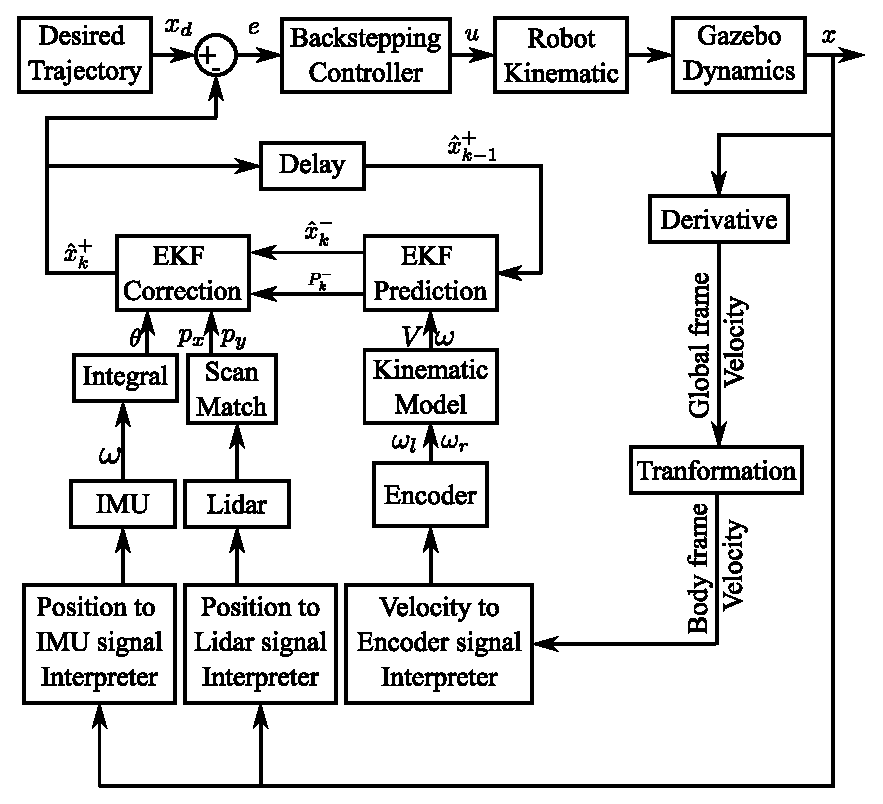
\includegraphics[scale=1]{images/imagess/5cont-propose_arch.eps} 
	\caption{Sensor Fusion Localization and control architecture}
	\label{fig:Sensor Fusion Localization and control architecture}
\end{figure}
% Figure Image =============================================================================